\documentclass[openany, a4paper,12pt, oneside]{article}
\usepackage[utf8]{inputenc}
\usepackage[brazil]{babel}
\usepackage{amsfonts}
\usepackage{multirow}
\usepackage{amssymb}
\usepackage{graphicx}
\usepackage{subfigure}
\usepackage{units}
\usepackage{placeins}
\usepackage{listings}
\usepackage{tabularx,colortbl}
\usepackage{fancyhdr,lastpage}
\usepackage{color}
\usepackage{algorithm}
\usepackage{algpseudocode}
\usepackage{anysize}
\marginsize{3.0cm}{2.5cm}{3.0cm}{2.5cm}
\oddsidemargin 0.0cm
\usepackage{transparent}
\usepackage{eso-pic}
\usepackage[T1]{fontenc}
\usepackage{lscape}
\usepackage{lettrine}
\usepackage{etoolbox}
\usepackage{abntex2cite}
\usepackage{cite}
\usepackage{graphicx}
\usepackage{breakcites}


\apptocmd{\thebibliography}{\csname phantomsection\endcsname\addcontentsline{toc}{chapter}{\bibname}}{}{}

\newcolumntype{L}[1]{>{\raggedright\let\newline\\\arraybackslash\hspace{0pt}}m{#1}}
\newcolumntype{C}[1]{>{\centering\let\newline\\\arraybackslash\hspace{0pt}}m{#1}}
\newcolumntype{R}[1]{>{\raggedleft\let\newline\\\arraybackslash\hspace{0pt}}m{#1}}
\usepackage{rotating}
\usepackage{setspace}
\usepackage[titletoc]{appendix}
\usepackage{pdfpages}
\usepackage{units}

\begin{document}
\pagestyle{empty}
\begin{flushright}
	\noindent\rule{15cm}{0.4pt}\\[0.5cm]
	\textbf{{ \LARGE Projeto de Conclus\~{a}o de Curso}}\\[0.1cm]
	\noindent\rule{15cm}{0.4pt}\\[7cm]
	\textbf{{ \Large Auxílio a tomada de decisão para ambientes na nuvem}}\\[4cm]
\end{flushright}

\begin{center}	
	\textbf{\large Alexandre Gouveia}\\[3cm]	
	
	\textbf{\large \'{A}rea de Concentra\c{c}\~{a}o:} Análise de desempenho de sistemas\\	
	\textbf{\large Orientador(a):} Carlos Julian Menezes Araújo\\[2cm]
	\vfill
	\textsc{Recife, Junho/2018}.
\end{center}
\pagebreak
\pagenumbering{gobble}

\begin{center}	
	\textbf{\textsc{\large Documento de Projeto de Pesquisa}}\\[1cm]
\end{center}



\section{Introdução}
\label{intro}

A computação em nuvem emergiu como um paradigma de computação para fornecer recursos
sob demanda (por exemplo, infraestrutura, plataforma,~\textit{software} dentre outros.) para usuários semelhantes
a concessionárias de serviços públicos (por exemplo, água, eletricidade e gás)~\cite{Sanket2018}.
Esse paradigma tem se tornado uma solução interessante para muitas empresas que buscam
escalabilidade e flexibilidade para o provimento de seus serviços. Essa mudança reflete
também nas empresas que buscam reduzir custos com a aquisição e manutenção dos recursos de computação,
assim como, almejam aumentar a eficiência no provimento do serviço.

Com o passar do tempo a utilização da computação em nuvem vem crescendo dentro
das empresas, onde em $2016$ a adoção de nuvem híbridas cresceu de $19\%$ para $57\%$~\cite{Forbes}.
A computação em nuvem tem por objetivo entregar recursos sob demanda para seus
usuários. Dentre os modelos de nuvem temos: a nuvem pública em que empresas provedoras
oferecem serviços através da Internet pública, tornando-o disponível para quem quiser
utilizar ou comprar; na nuvem privada os serviços são disponibilizados através da
Internet ou de uma rede interna, permitindo um controle adicional ou customizações de recursos dedicados sobre uma estrutura computacional hospedada na
empresa. A nuvem privada também permite um nível maior de segurança. Há um terceiro
modelo que é conhecido como nuvem híbrida, que combina os modelos supracitados permitindo
que dados e aplicações sejam compartilhados entre si, quando a demanda flutua, a computação
em nuvem híbrida permite de forma transparente escalar a infraestrutura local da empresa \cite{Ms}.


Os serviços providos pela nuvem podem ser divididos em três grupos principais:
\textit{Software as a Service} (SaaS) que provê \textit{software} e aplicações através da Internet,
\textit{Plataform as a service} (PaaS) que entrega aos usuários um ambiente para desenvolver, gerenciar e
entrega aplicações e \textit{Infraestructure as a Service}(IaaS) que provê acesso a recursos
computacionais como servidores, \textit{storages} e redes \cite{IBM}.
No mercado de serviços em nuvem podemos citar um grande número de empresas
oferecendo inúmeras opções de serviço dentre as quais temos: Amazon (AWS), Embratel,
Microsoft (Azure), Google (Google cloud), dentre outros. Assim, com uma grande diversidade de serviços
ofertados na nuvem, a tarefa de escolher uma opção adequada se torna bastante difícil para o usuário.
Adicionalmente, podemos também citar diversos critérios associados a cada serviço, como custo,
desempenho, confiabilidade, disponibilidade dentre outros, o que torna esta uma atividade ainda mais trabalhosa.

Esta questão de qual serviço em nuvem escolher pode ser incluída dentro dos
problemas de tomada de decisão multicritério, onde diversos fatores devem ser
considerados para que se escolha uma solução que satisfaça os critérios estabelecidos. Dentre os métodos para tomada de
decisão multicritério alguns dos mais utilizados são o \textit{Preference Ranking Organization
Method for Enrichment Evaluation} (PROMETHEE) e o \textit{Technique for Order Performance by
Similarity to Ideal Solution} (TOPSIS) \cite{Javeed}.


Este trabalho tem por objetivo auxiliar usuários no processo de tomada de decisão, mitigando o conflito de interesse na escolha de um
serviço em nuvem (pública ou privada). O presente trabalho está dividido nas seguintes seções: a
Seção~\ref{sec-prob} apresenta o problema de pesquisa, Seção~\ref{sec-just} descreve a justificativa,
Seção~\ref{sec-obj} apresenta o objetivo geral e específicos , Seção~\ref{sec-pesq} apresenta as etapas de pesquisa realizadas , Seção \ref{sec-cron} apresenta o cronograma das contendo as atividades.

\section{Problema de Pesquisa}
\label{sec-prob}

%Tendo em vista a crescente oferta de empresas que provem serviços na nuvem como
%escolher um serviço na nuvem que melhor atenda as necessidade da empresa tendo em
%vista que esta é uma atividade que requer muito tempo devido a quantidade de fatores
%envolvidos nesta escolha.


O problema fundamental tratado neste projeto de graduação é abordado na seguinte pergunta: Como mitigar
o processo de seleção e escolha de serviços computacionais em nuvens considerando políticas de prestação de serviços
com restrição de orçamento, garantindo níveis aceitáveis de disponibilidade e desempenho?




\section{Justificativa}
\label{sec-just}

O crescente número de informações sobre serviços ofertados na nuvem e a necessidade de utilizá-los
no processo decisório fez com que surgissem diversas pesquisas com o intuito de auxiliar
gestores e usuários na tomada de decisão\cite{Saurabh,Whaiduzzaman,Alabool}.
Os métodos multicritérios de tomada de decisão surgiram como métodos de apoio para
resolução de problemas em que existem critérios conflitantes (por exemplo, custo e confiabilidade).
Assim, a tomada de decisão multicritério é uma abordagem que pode auxiliar na seleção de diferentes alternativas 
que consideram um conjunto de critérios e também confere ao processo clareza e transparência \cite{SABAEI, Kroenke}. 

A utilização de métodos multicritérios ocorre pelo fato de que não há, em geral, processos
decisórios que atendam simultaneamente a todos os critérios em análise. Assim, considerando
diversos critérios que precisam ser levados em conta no processo de seleção de serviços
em nuvem, métodos de decisão multicritério se tornam uma escolha interessante na seleção
desses serviços. Tais métodos também auxiliam na redução dos riscos que são associados ao processo
de escolha como custo-necessidade.

%Com este trabalho espera-se que seja confeccionada uma ferramenta que dado uma entrada
%contendo informações sobre os serviços em nuvem disponível e classificá-los de acordo
%com seus atributos.

No trabalho proposto por Kittur \cite{Javeed} foi realizado um estudo de caso para se encontrar
o melhor horário para geração de energia em um dia específico. Foram utilizados os atributos vento, \textit{combine heat power}, \textit{utility} e custo. Foram aplicados os métodos \textit{PROMETHEE} e \textit{TOPSIS} e para determinar o peso dos atributos foi utilizado o \textit{Analytic Hierarchy Process}(AHP).
Segundo os resultados obtidos neste estudo de caso tanto \textit{PROMETHEE} quanto o \textit{TOPSIS} foram capazes de encontrar a melhor solução porém em horários distintos.

Em \cite{Saurabh}, o trabalho teve por objetivo a criação de um \textit{framework} utilizando o
\textit{Analytic Hierarchy Process} (AHP) para a comparação de serviços na nuvem. Esta comparação
foi feita por meio de atributos propostos pelo \textit{Cloud Service Measurent Index Consortium}(CSMIC)
como custo, agilidade, segurança, desempenho, garantia(assurance) e accountability. Os autores acreditam
que este \textit{framework} representa um passo  importante no que diz respeito a seleção de serviços
na nuvem. E que por utilizar as técnicas citadas neste trabalho os provedores de serviço na nuvem podem
comparar sua oferta de serviço com os concorrentes.

O trabalho proposto por \cite{SABAEI} tem o objetivo de realizar uma revisão dos métodos de decisão
multicritério, avaliá-los e realizar uma análise crítica. Os autores constataram a existência de
uma lacuna no que diz repeito a uma comparação entre os métodos de tomada de decisão.E com este
trabalho eles conseguiram preencher esta lacuna ao apresentar uma análise dos diferentes métodos
de tomada de decisão. Segundo os resultados obtidos no estudo o método \textit{Analytic Hierarchy Proces} (AHP)
pode providenciar uma solução robusta pôr levar em consideração as preferências do usuário em primeirow lugar.

O trabalho proposto por \cite{Arese} teve por objetivo a utilização do método de decisão multicritério \textit{TOPSIS} para definir quais as métricas mais importantes para seleção de docentes dentro de uma instituição de ensino superior. Cada alternativa é uma característica usada para avaliar o docente e seus atributos são uma nota dada por coordenadores de curso(no total 10 coordenadores). No que diz respeito aos resultados dos 8 atributos mais importantes de acordo com a pesquisa apenas metade deles é considerada pelo MEC como quesito para avaliar as instituições de ensino médio e as 2 alternativas apontadas como mais importantes segundo a pesquisa não são consideradas pelo MEC(Experiência como docente e empatia).

No trabalho feito por \cite{Kroenke}, foi utilizado o método para tomada de decisão multicritério AHP para a seleção de fornecedores. Este trabalho foi desenvolvido com base em uma pesquisa de campo, por meio de um estudo de caso. Neste trabalho a tomada de decisão foi dividida em três etapas sendo elas: parametrização do modelo que inicia com a escolha dos funcionário que estarão ligados ao processo de tomada de decisão, simulação computacional baseado no modelo AHP, onde a partir dos dados coletados será gerada uma planilha com as alternativas de serviços a partir da qual será gerado um \textit{ranking} das alternativas. E por fim os funcionários selecionados na etapa 1 irão selecionar as alternativas com base nos resultados da etapa 2. Os autores ressaltam que apesar de se utilizar um método de decisão a palavra final sobre qual fornecedor escolher cabe ao gestor.

No estudo feito por \cite{Whaiduzzaman} teve por objetivos realizar uma análise comparativa entre os métodos de análise de decisão multicritério(MCDA), apresentar uma taxonomia destes métodos através de uma revisão literária e analisar e resumir a seleção de serviços de computação em nuvem em diferentes cenários. Ele conclui que os MCDA tem um grande efeito e importância nos cenários de tomada de decisão multicritério. Este estudo realizado apresenta as vantagens e desvantagens bem como aplicações destes métodos analisados. 

\section{Objetivos}
\label{sec-obj}

\textbf{Objetivo Geral:\\} 
	

	Adotar métodos baseados em análise multi-critério para auxiliar usuários no processo de tomada de decisão
	para selecionar serviços em nuvem (pública ou privada), através de métricas como
	agilidade, desempenho, custo, \textit{accountability}, segurança e garantia (\textit{assurance}).
	\\
	

	
\textbf{Objetivos Específicos:\\}


\begin{enumerate}

    \item Implementar uma abordagem baseada em algoritmos multi-critérios que auxiliem usuários de serviços na nuvem na seleção de serviços.

    \item Realizar um estudo de caso visando demonstrar a aplicabilidade da ferramenta no processo de tomada de decisão.


	
	
\end{enumerate}

\section{Etapas da Pesquisa}
\label{sec-pesq}


Esta proposta fará uma pesquisa exploratória no intuito de identificar características dos trabalhos
realizados sobre a atividade de seleção de serviços em nuvem, assim como, buscará evidenciar os métodos
mais utilizados na literatura. A pesquisa será realizada por meio de uma revisão bibliográfica, na qual
serão levantados artigos publicados em periódicos e conferências relacionados a temas de computação em
nuvem, métodos multicritério e tomada de decisão. Serão utilizadas como palavras-chave:
seleção de serviços em nuvem, desempenho, disponibilidade, processo de seleção, multicritérios.
A Figura~\ref{fig:metodologia} ilustra as etapas da metodologia adotada nesta proposta e contextualiza
o ambiente no qual este trabalho está inserido, destacando suas principais atividades.

\begin{figure}[h]
    \centering
    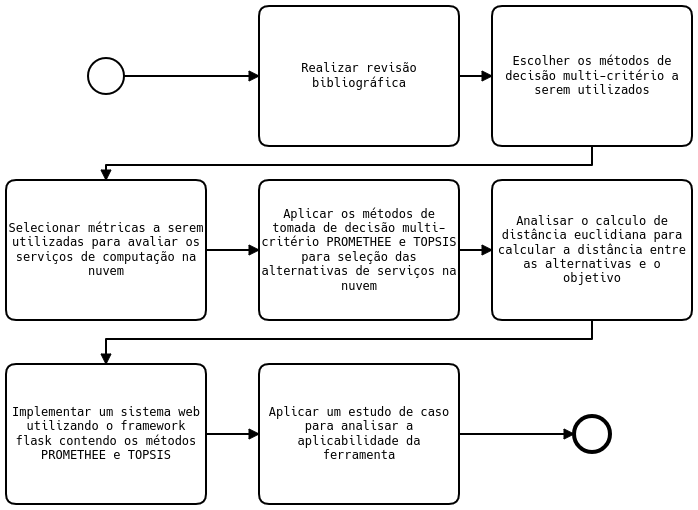
\includegraphics[width=\textwidth]{fluxo}
    \caption{Fluxograma das etapas de pesquisa.}
    \label{fig:metodologia}
\end{figure}


\begin{enumerate}
    \item Realizar revisão bibliográfica;
    \item Escolher os métodos de decisão multi-critério a serem utilizados;
    \item Selecionar métricas a serem utilizadas para avaliar os serviços de computação na nuvem;
    \item Analisar os métodos de tomada de decisão multi-critério \textit{PROMETHEE} e \textit{TOPSIS} para seleção das alternativas de serviços na nuvem;
    \item Analisar o cálculo de distância euclidiana para calcular a distância entre as alternativas e o objetivo;
    \item Implementar um sistema web utilizando o \textit{framework flask} contendo os métodos \textit{PROMETHEE} e \textit{TOPSIS};
    \item Realizar um estudo de caso para analisar a aplicabilidade do sistema;
    
\end{enumerate}

\section{Cronograma}
\label{sec-cron}


\begin{figure}[h]
    \centering
    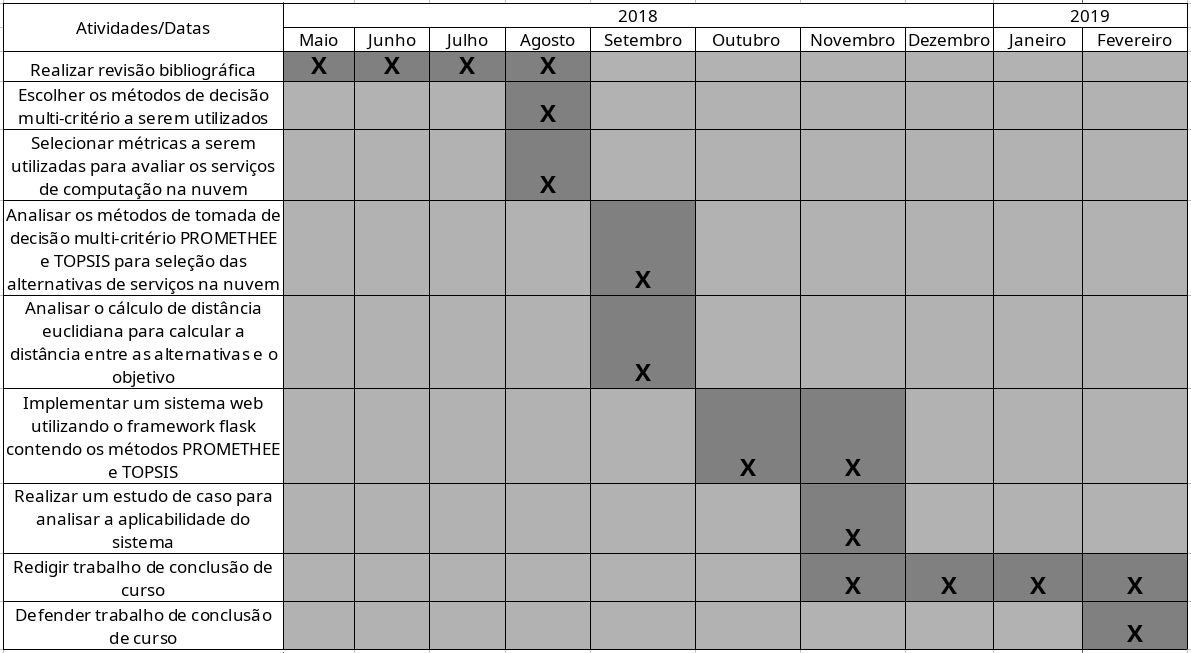
\includegraphics[width=\textwidth]{cronograma.png}
    \caption{Cronograma das atividades}
    \label{fig:my_label}
\end{figure}

\bibliographystyle{abntex2-alf}
\bibliography{bibliography}

\end{document}
